
    \centering
    \tikzsetnextfilename{ejercicio28_figura} 
    
    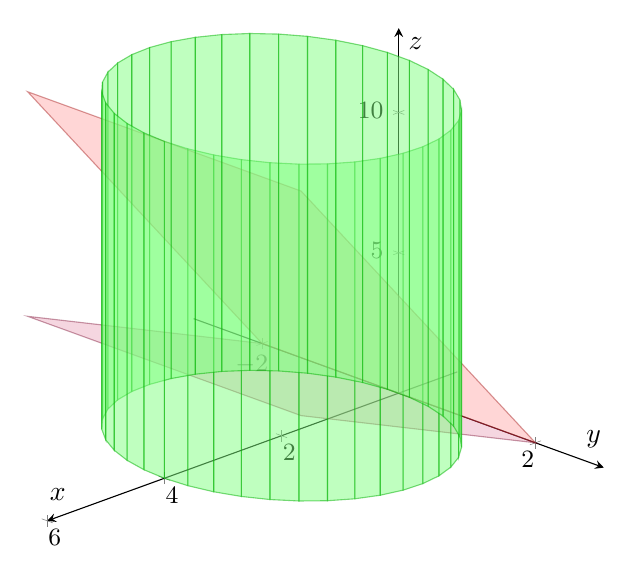
\begin{tikzpicture}
        \begin{axis}[
            view={135}{30}, % Ajustado para ver bien la inclinación de los planos
            width=12cm,
            height=10cm,
            grid=major,
            xmin=-1, xmax=6,
            ymin=-3, ymax=3,
            zmin=0, zmax=13,
            xlabel={$x$},
            ylabel={$y$},
            zlabel={$z$},
            axis lines=center,
            ticklabel style={font=\small},
        ]

        % Plano g: z = x (Violeta)
        \addplot3[
            surf,
            domain=0:4,
            y domain=-2:2,
            samples=2,
            color=purple!40,
            opacity=0.4,
            faceted color=purple!60!black,
        ] {x};

        % Plano h: z = 3x (Rojo)
        \addplot3[
            surf,
            domain=0:4,
            y domain=-2:2,
            samples=2,
            color=red!40,
            opacity=0.4,
            faceted color=red!60!black,
        ] {3*x};

        % Cilindro f: (x-2)^2 + y^2 = 4 (Verde)
        % Parametrización: x = 2 + 2*cos(t), y = 2*sin(t)
        \addplot3[
            surf,
            domain=0:360, % ángulo t
            y domain=0:12, % altura z (hasta el máximo de 3x)
            samples=40,
            samples y=2,
            color=green!50,
            opacity=0.5,
            faceted color=green!70!black,
        ]
        ({2 + 2*cos(x)}, {2*sin(x)}, {y});

        \end{axis}
    \end{tikzpicture}
    \caption{Representación de la región pedida.  \href{https://www.geogebra.org/m/uhgycge3}{Ver en GeoGebra}}
